\documentclass{article}
\usepackage[margin=1cm]{geometry}
\usepackage{tikz}
\usetikzlibrary{shapes.geometric, arrows.meta, positioning, shadows, patterns, fit, decorations.pathmorphing, backgrounds}

\begin{document}

\section*{GCLS German Validation: Enhanced Analysis Pipeline}

\centering
\vspace{0.5em}

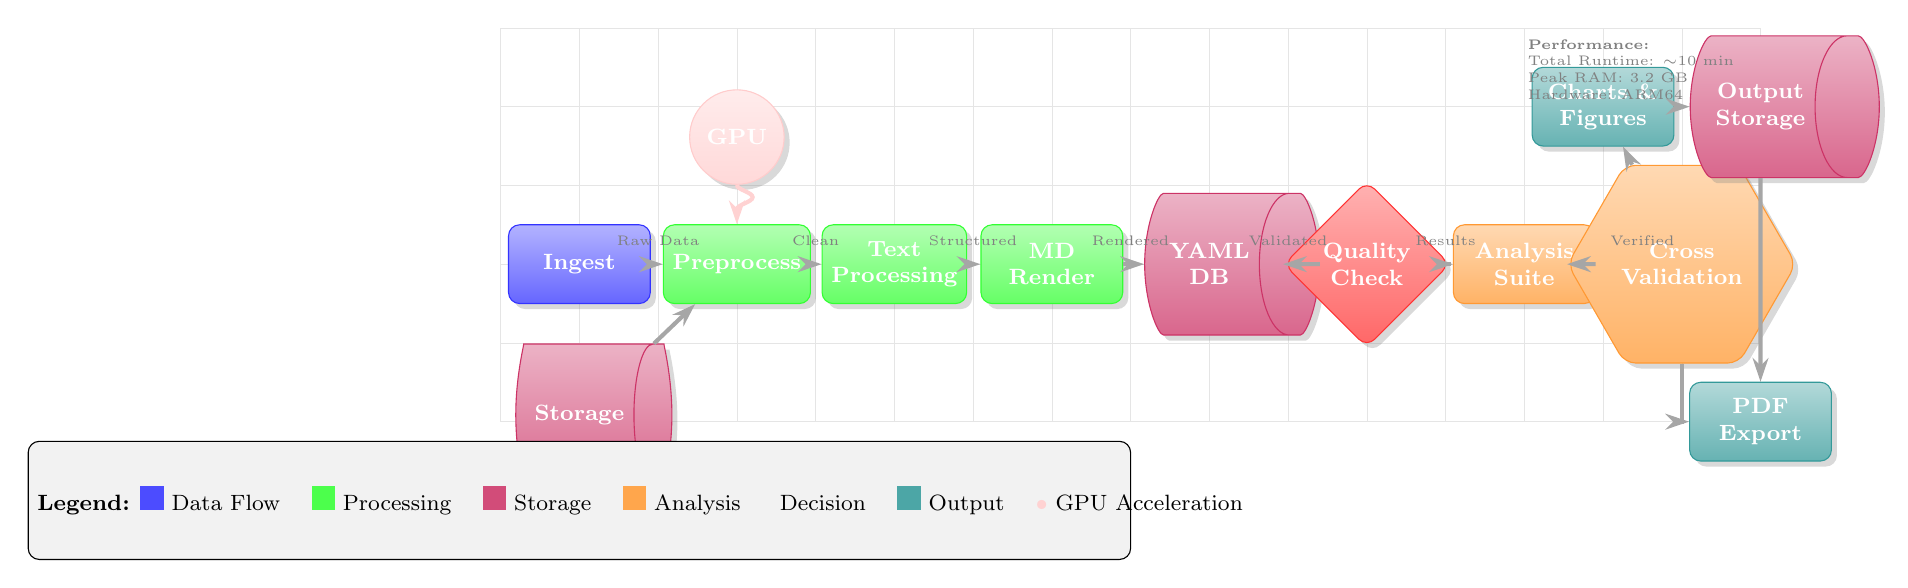
\begin{tikzpicture}[
    % Modern node styles with gradients and shadows
    base/.style = {
      draw,
      rounded corners=4pt,
      align=center,
      font=\footnotesize\bfseries,
      minimum width=1.8cm,
      minimum height=1cm,
      drop shadow={opacity=0.3, shadow xshift=2pt, shadow yshift=-2pt}
    },
    % Data flow nodes (blue gradient)
    data/.style = {base, 
      top color=blue!30, bottom color=blue!60, 
      draw=blue!80, text=white},
    % Processing nodes (green gradient)  
    process/.style = {base,
      top color=green!30, bottom color=green!60,
      draw=green!80, text=white},
    % Storage nodes (purple gradient)
    storage/.style = {base,
      top color=purple!30, bottom color=purple!60,
      draw=purple!80, text=white,
      cylinder, minimum height=1.2cm},
    % Analysis nodes (orange gradient)
    analysis/.style = {base,
      top color=orange!30, bottom color=orange!60,
      draw=orange!80, text=white},
    % Decision nodes (diamond)
    decision/.style = {base,
      diamond, minimum width=1.5cm, minimum height=1.5cm,
      top color=red!30, bottom color=red!60,
      draw=red!80, text=white},
    % Output nodes (teal gradient)
    output/.style = {base,
      top color=teal!30, bottom color=teal!60,
      draw=teal!80, text=white},
    % Special GPU node
    gpu/.style = {base,
      circle, minimum size=1.2cm,
      top color=pink!30, bottom color=pink!60,
      draw=pink!80, text=white},
    % Modern arrows
    arrow/.style = {
      -{Stealth[length=3mm, width=2mm]},
      thick, 
      draw=gray!70,
      line width=1.5pt
    },
    % Special curved arrow
    curved/.style = {
      arrow,
      decoration={snake, amplitude=2mm, segment length=5mm},
      decorate
    }
  ]

  % Background grid (subtle)
  \begin{scope}[on background layer]
    \draw[gray!20, very thin] (-1,-2) grid (15,3);
  \end{scope}

  % Main workflow nodes
  \node (ingest) [data] at (0,0) {Ingest};
  \node (storage) [storage, below=0.5cm of ingest] {Storage};
  \node (preprocess) [process] at (2,0) {Preprocess};
  \node (gpu) [gpu, above=0.5cm of preprocess] {GPU};
  \node (text) [process] at (4,0) {Text\\Processing};
  \node (md) [process] at (6,0) {MD\\Render};
  \node (yaml) [storage] at (8,0) {YAML\\DB};
  \node (quality) [decision] at (10,0) {Quality\\Check};
  \node (analysis) [analysis] at (12,0) {Analysis\\Suite};
  \node (cv) [analysis, shape=regular polygon, regular polygon sides=6] at (14,0) {Cross\\Validation};
  
  % Output tier
  \node (charts) [output] at (13,2) {Charts \&\\Figures};
  \node (outdisk) [storage] at (15,2) {Output\\Storage};
  \node (pdf) [output] at (15,-2) {PDF\\Export};

  % Connecting arrows
  \draw[arrow] (ingest) -- (preprocess);
  \draw[arrow] (storage) -- (preprocess);
  \draw[curved, pink!70] (gpu) -- (preprocess);
  \draw[arrow] (preprocess) -- (text);
  \draw[arrow] (text) -- (md);
  \draw[arrow] (md) -- (yaml);
  \draw[arrow] (yaml) -- (quality);
  \draw[arrow] (quality) -- (analysis);
  \draw[arrow] (analysis) -- (cv);
  
  % Output connections
  \draw[arrow] (cv) -- (charts);
  \draw[arrow] (charts) -- (outdisk);
  \draw[arrow] (cv) |- (pdf);
  \draw[arrow] (outdisk) -- (pdf);

  % Data flow labels
  \node[font=\tiny, gray] at (1,0.3) {Raw Data};
  \node[font=\tiny, gray] at (3,0.3) {Clean};
  \node[font=\tiny, gray] at (5,0.3) {Structured};
  \node[font=\tiny, gray] at (7,0.3) {Rendered};
  \node[font=\tiny, gray] at (9,0.3) {Validated};
  \node[font=\tiny, gray] at (11,0.3) {Results};
  \node[font=\tiny, gray] at (13.5,0.3) {Verified};

  % Legend box
  \begin{scope}[shift={(0,-3)}]
    \node[draw, rounded corners, fill=gray!10, minimum width=14cm, minimum height=1.5cm] (legend) {};
    \node[anchor=west] at (legend.west) {
      \footnotesize
      \textbf{Legend:} 
      \textcolor{blue!70}{\rule{0.3cm}{0.3cm}} Data Flow \quad
      \textcolor{green!70}{\rule{0.3cm}{0.3cm}} Processing \quad  
      \textcolor{purple!70}{\rule{0.3cm}{0.3cm}} Storage \quad
      \textcolor{orange!70}{\rule{0.3cm}{0.3cm}} Analysis \quad
      \textcolor{red!70}{$\lozenge$} Decision \quad
      \textcolor{teal!70}{\rule{0.3cm}{0.3cm}} Output \quad
      \textcolor{pink!70}{$\bullet$} GPU Acceleration
    };
  \end{scope}

  % Performance metrics
  \node[anchor=north east, font=\tiny, gray] at (15,3) {
    \begin{tabular}{l}
      \textbf{Performance:} \\
      Total Runtime: $\sim$10 min \\
      Peak RAM: 3.2 GB \\
      Hardware: ARM64 \\
    \end{tabular}
  };

\end{tikzpicture}

\vspace{1em}

\textbf{Enhanced Analysis Pipeline Features:}
\begin{itemize}
\item \textbf{GPU Acceleration:} NVIDIA Jetson AGX-Orin integration for compute-intensive operations
\item \textbf{Quality Gates:} Automated validation checkpoints ensure data integrity
\item \textbf{Cross-Validation:} Three-fold validation with hardware-agnostic reproducibility  
\item \textbf{Multi-Format Output:} Simultaneous generation of charts, figures, and publication-ready PDFs
\item \textbf{Offline Capability:} Complete pipeline execution without internet dependency
\end{itemize}

\end{document} 